\documentclass[11pt,letterpaper]{article}

%% ── Packages ─────────────────────────────────────────────────────────────────
\usepackage[margin=1in]{geometry}
\usepackage{amsmath}
\usepackage{amssymb}
\usepackage{xcolor}
\usepackage[most]{tcolorbox}
\usepackage{enumitem}
\usepackage{booktabs}
\usepackage{array}
\usepackage{siunitx}
\usepackage{graphicx}
\usepackage{fancyhdr}
\usepackage{titlesec}
\usepackage{hyperref}
\usepackage{multicol}
\usepackage{pgfplots}
\usepackage[american,siunitx]{circuitikz}
\usepackage{float}
\usepackage{parskip}
\usepackage{microtype}
\usepackage{caption}

\pgfplotsset{compat=1.18}
\usetikzlibrary{arrows.meta, positioning, calc}

%% ── Colors ───────────────────────────────────────────────────────────────────
\definecolor{navyblue}{RGB}{20,52,120}
\definecolor{skyblue}{RGB}{210,230,255}
\definecolor{lightgray}{RGB}{245,245,245}
\definecolor{gold}{RGB}{180,140,0}
\definecolor{darkgold}{RGB}{120,90,0}
\definecolor{answergreen}{RGB}{0,100,50}
\definecolor{answerbg}{RGB}{230,255,240}
\definecolor{warnbg}{RGB}{255,248,220}
\definecolor{warnborder}{RGB}{200,150,0}
\definecolor{exbg}{RGB}{240,245,255}
\definecolor{quizbg}{RGB}{255,250,240}
\definecolor{quizborder}{RGB}{180,130,0}
\definecolor{keybg}{RGB}{225,240,225}
\definecolor{tiplabel}{RGB}{0,80,140}
\definecolor{tipbg}{RGB}{235,245,255}

%% ── tcolorbox styles ─────────────────────────────────────────────────────────
\tcbuselibrary{skins,breakable,theorems}

\newtcolorbox{conceptbox}[1]{
  breakable,
  colback=skyblue!40,
  colframe=navyblue,
  fonttitle=\bfseries\color{white},
  coltitle=white,
  attach boxed title to top left={yshift=-2mm,xshift=4mm},
  boxed title style={colback=navyblue, sharp corners},
  title={#1},
  sharp corners=south,
  top=6pt, bottom=6pt,
}

\newtcolorbox{examplebox}[1]{
  breakable,
  colback=exbg,
  colframe=navyblue!60,
  fonttitle=\bfseries\color{navyblue},
  coltitle=navyblue,
  attach boxed title to top left={yshift=-2mm,xshift=4mm},
  boxed title style={colback=skyblue, colframe=navyblue!60, sharp corners},
  title={#1},
  sharp corners=south,
  top=6pt,bottom=6pt,
}

\newtcolorbox{quizbox}[1]{
  breakable,
  colback=quizbg,
  colframe=quizborder,
  fonttitle=\bfseries\color{darkgold},
  coltitle=darkgold,
  attach boxed title to top left={yshift=-2mm,xshift=4mm},
  boxed title style={colback=warnbg, colframe=quizborder, sharp corners},
  title={#1},
  sharp corners=south,
  top=6pt, bottom=6pt,
}

\newtcolorbox{answerbox}[1]{
  breakable,
  colback=answerbg,
  colframe=answergreen!70,
  fonttitle=\bfseries\color{answergreen},
  coltitle=answergreen,
  attach boxed title to top left={yshift=-2mm,xshift=4mm},
  boxed title style={colback=answerbg, colframe=answergreen!70, sharp corners},
  title={#1},
  sharp corners=south,
  top=6pt, bottom=6pt,
}

\newtcolorbox{tipbox}{
  breakable,
  colback=tipbg,
  colframe=tiplabel!60,
  fonttitle=\bfseries\color{tiplabel},
  title={Tip},
  sharp corners=south,
  top=5pt, bottom=5pt,
}

\newtcolorbox{warnbox}{
  breakable,
  colback=warnbg,
  colframe=warnborder,
  fonttitle=\bfseries\color{darkgold},
  title={Common Mistake},
  sharp corners=south,
  top=5pt, bottom=5pt,
}

%% ── Section formatting ───────────────────────────────────────────────────────
\titleformat{\section}{\large\bfseries\color{navyblue}}{\thesection}{1em}{}[\titlerule]
\titleformat{\subsection}{\normalsize\bfseries\color{navyblue!80}}{\thesubsection}{1em}{}
\titleformat{\subsubsection}{\normalsize\bfseries\color{navyblue!60}}{\thesubsubsection}{1em}{}

%% ── Header / footer ──────────────────────────────────────────────────────────
\pagestyle{fancy}
\fancyhf{}
\lhead{\small\color{navyblue}\textbf{LED Circuit Design} --- Study Guide}
\rhead{\small\color{navyblue}\leftmark}
\rfoot{\small Page \thepage}
\lfoot{\small\color{gray}\today}
\renewcommand{\headrulewidth}{0.4pt}

%% ── Hyperref ─────────────────────────────────────────────────────────────────
\hypersetup{colorlinks=true,linkcolor=navyblue,urlcolor=navyblue}

%% ── siunitx ──────────────────────────────────────────────────────────────────
\sisetup{per-mode=symbol}

%% ── Misc helpers ─────────────────────────────────────────────────────────────
\newcolumntype{C}[1]{>{\centering\arraybackslash}p{#1}}
\newcolumntype{L}[1]{>{\raggedright\arraybackslash}p{#1}}
\newcommand{\ohm}{\,\si{\ohm}}
\newcommand{\volt}{\,\si{V}}
\newcommand{\mA}{\,\si{mA}}
\newcommand{\mW}{\,\si{mW}}
\newcommand{\Watt}{\,\si{W}}
\newcommand{\Vf}{V_f}
\newcommand{\Vcc}{V_{CC}}
\newcommand{\Imax}{I_{max}}
\newcommand{\Iled}{I_{LED}}
\newcommand{\blank}{\underline{\hspace{2cm}}}

%% ── Exercise counter ─────────────────────────────────────────────────────────
\newcounter{exercise}
\newcommand{\exercise}{\stepcounter{exercise}\textbf{Exercise~\theexercise.}~}

\newcounter{quiz}
\newcommand{\quizq}{\stepcounter{quiz}\textbf{Q\thequiz.}~}

%% ─────────────────────────────────────────────────────────────────────────────
\begin{document}

%% ── Title page ───────────────────────────────────────────────────────────────
\begin{titlepage}
  \centering
  \vspace*{1.5cm}
  {\Huge\bfseries\color{navyblue} Designing with LEDs\par}
  \vspace{0.4cm}
  {\Large A Practical Study Guide\par}
  \vspace{0.3cm}
  {\large\color{gray} Selecting components, calculating resistors,\\
   and matching circuits to design goals\par}
  \vspace{2.5cm}

  %% Simple LED circuit illustration
  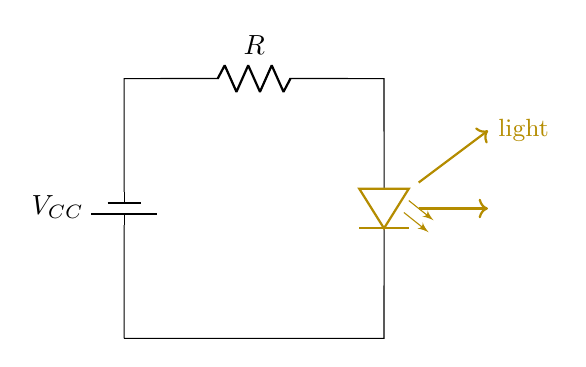
\begin{tikzpicture}[scale=1.1]
    \ctikzset{resistors/scale=0.8, diodes/scale=0.9}
    \draw (0,0) to[battery1, l=$V_{CC}$] (0,3)
                to[R, l=$R$] (3,3)
                to[led, color=gold] (3,0)
                -- (0,0);
    \draw[->, thick, gold] (3.4,1.8) -- (4.2,2.4) node[right,gold]{\small light};
    \draw[->, thick, gold] (3.4,1.5) -- (4.2,1.5) node[right,gold]{\small };
  \end{tikzpicture}

  \vspace{2cm}
  {\normalsize
    \begin{tabular}{rl}
      \textbf{Topics covered:} & LED physics, forward voltage, current limiting \\
      & Ohm's law applied to LED circuits \\
      & Selecting operating current (Low / Medium / High) \\
      & Resistor power ratings and package sizing \\
      & Matching LEDs to voltage and current budgets \\
      & Interpreting datasheets and handling uncertainty \\
    \end{tabular}
  }
  \vfill
  {\small\color{gray} Exercises and worked examples throughout.
  Answer key in Appendix~A.}
\end{titlepage}

\tableofcontents
\newpage

%%=============================================================================
\section{What Is an LED?}
%%=============================================================================
\markboth{Section 1 --- What Is an LED?}{}

A \textbf{Light Emitting Diode (LED)} is a semiconductor device that emits light when
current flows through it in the forward direction. Unlike a resistor, whose resistance
is fixed by Ohm's law, an LED presents a nearly constant \emph{voltage drop} when
conducting, and is very sensitive to the current flowing through it.

\begin{conceptbox}{Key LED Properties}
\begin{itemize}[leftmargin=1.5em]
  \item \textbf{Forward Voltage ($\Vf$):} The voltage drop across the LED when it
    is conducting. This is fixed by the LED's chemistry and color, not by the circuit.
    Typical values range from about 1.8\volt{} (red) to 4.0\volt{} (violet/UV).
  \item \textbf{Forward Current ($\Iled$):} The current flowing through the LED.
    Brightness is approximately proportional to current.
  \item \textbf{Maximum Current ($\Imax$):} The absolute maximum current the LED can
    handle continuously without damage. Never exceed this.
  \item \textbf{Reverse breakdown:} LEDs are destroyed if significant voltage is
    applied backwards. Always connect the anode ($+$) toward the positive supply.
\end{itemize}
\end{conceptbox}


\subsection{The LED's I--V Curve and the Load Line}

Unlike a resistor, the LED does \emph{not} obey Ohm's law directly. Its
current-versus-voltage relationship is \textbf{highly nonlinear}: below $\Vf$ almost
no current flows; above it, current rises exponentially and extremely steeply.
This behaviour is described by the \emph{diode equation}, but for practical circuit
design the key points are:

\begin{itemize}[leftmargin=2em]
	\item The curve is nearly \textbf{flat near zero} --- the LED is essentially an
	open circuit below its threshold voltage.
	\item The curve becomes \textbf{nearly vertical above $\Vf$} --- once conducting,
	a tiny increase in voltage produces a huge increase in current.
	\item The steepness means that connecting an LED directly to a fixed voltage source
	is dangerous: with no resistance to limit current, the LED sits on the vertical
	part of its curve and draws as much current as the source can supply, burning out
	in milliseconds.
\end{itemize}

\subsubsection*{The Load Line}

The series resistor $R$ imposes its own constraint on the circuit, described by
a straight line called the \textbf{load line}. By Kirchhoff's voltage law, whatever
voltage the LED takes ($V_{LED}$), the resistor gets the rest:
\[ V_R = \Vcc - V_{LED} \]
and the current through the resistor is $I = V_R / R$, so:
\[ I = \frac{\Vcc - V_{LED}}{R} \]

This is a straight line on the I--V axes. It has two easy-to-find endpoints:
\begin{itemize}[leftmargin=2em]
	\item \textbf{X-intercept} (current = 0): $V_{LED} = \Vcc$.
	If no current flows, the full supply appears across the LED.
	\item \textbf{Y-intercept} (voltage across LED = 0): $I = \Vcc / R$.
	If the LED were a short circuit, the resistor would limit current to $\Vcc/R$.
\end{itemize}

\subsubsection*{The Operating Point}

The LED and resistor are in the same series loop, so they must simultaneously satisfy
\emph{both} constraints --- the LED's I--V curve \emph{and} the load line. The only
point that satisfies both at once is where the two lines \textbf{intersect}.
This intersection is the \textbf{operating point}: the actual current and voltage
at which the circuit runs.

Graphically, you draw the LED curve and the load line on the same axes. The operating
point falls naturally on the steep part of the LED curve, in the region where
the curve is nearly vertical. This has an important consequence: the steep curve
means the operating point's \emph{current} is mostly controlled by the load line
(i.e.\ the resistor), while the \emph{voltage} is pinned near $\Vf$ by the LED.
This is exactly the behaviour we want --- the resistor sets the current, and the LED
self-selects its voltage.

\begin{figure}[H]
	\centering
	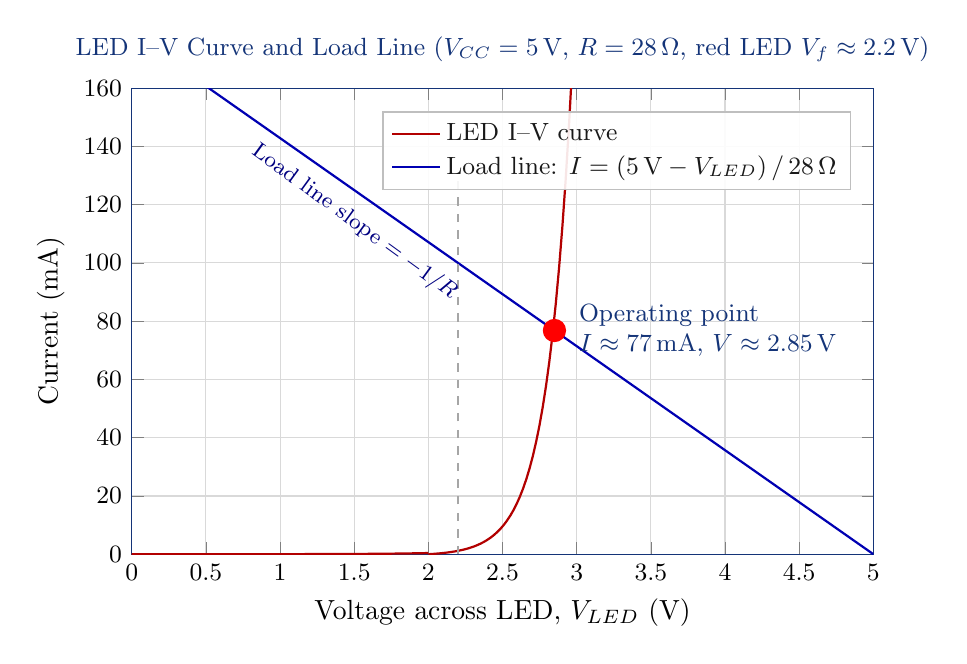
\begin{tikzpicture}
		\begin{axis}[
			width=11cm, height=7.5cm,
			xlabel={Voltage across LED, $V_{LED}$ (V)},
			ylabel={Current (mA)},
			xmin=0, xmax=5.0,
			ymin=0, ymax=160,
			grid=major, grid style={gray!30},
			xtick={0,0.5,1.0,1.5,2.0,2.5,3.0,3.5,4.0,4.5,5.0},
			ytick={0,20,40,60,80,100,120,140,160},
			title={\small LED I--V Curve and Load Line ($\Vcc=5$\,V, $R=28\,\Omega$,
				red LED $\Vf\approx2.2$\,V)},
			title style={color=navyblue},
			axis line style={navyblue},
			every tick label/.style={font=\small},
			legend style={at={(0.97,0.95)}, anchor=north east, font=\small,
				draw=gray!50, fill=white, fill opacity=0.9},
			legend cell align=left,
			]
			
			%% LED I-V curve
			\addplot[thick, red!70!black, domain=0:2.0, samples=60]
			{0.001*exp(3*(x-0))-0.001};
			\addlegendentry{LED I--V curve}
			\addplot[thick, red!70!black, domain=2.0:3.3, samples=60, forget plot]
			{0.5*exp(6*(x-2.0))-0.5};
			
			%% Load line: I = (5 - V_LED)/28 * 1000 mA
			\addplot[thick, blue!70!black, domain=0:5.0, samples=2]
			{(5.0 - x)/28 * 1000};
			\addlegendentry{Load line: $I=(5\,\text{V}-V_{LED})\,/\,28\,\Omega$}
			
			%% Vf dashed vertical line and label
			\draw[dashed, gray!70, thick] (axis cs:2.2,0) -- (axis cs:2.2,130);
			\node[below, font=\small, gray!80] at (axis cs:2.2,0) {$\Vf \approx 2.2$\,V};
			
			%% X-intercept label (Vcc)
			\node[below, font=\small, blue!70!black] at (axis cs:5.0,0) {$\Vcc$};
			
			%% Y-intercept label (Vcc/R)
			\node[left, font=\small, blue!70!black] at (axis cs:0,178)
			{$\frac{\Vcc}{R}$};
			
			%% Operating point
			\addplot[mark=*, mark size=4pt, color=red] coordinates {(2.85,76.8)};
			\node[right, font=\small, navyblue, align=left] at (axis cs:2.95,76.8)
			{Operating point\\$I \approx 77$\,mA, $V \approx 2.85$\,V};
			
			%% Load line slope label: placed on the line, rotated parallel to it,
			%% below and to the left of the operating point. No leader line.
			%% At x=1.5 on load line: I=(5-1.5)/28*1000 = 125 mA
			%% Label sits just below the line at that x position.
			\node[rotate=-36, font=\footnotesize, blue!50!black]
			at (axis cs:1.5,114) {Load line slope $= -1/R$};
			
		\end{axis}
	\end{tikzpicture}
	\caption{The LED I--V curve (red) and the load line (blue) for a $28\,\Omega$ resistor
		on a 5\,V supply. The load line runs from $(0,\,\Vcc/R)$ on the current axis to
		$(\Vcc,\,0)$ on the voltage axis. The operating point (filled circle) is the unique
		intersection: the only combination of current and voltage that satisfies both the
		LED's physics and Ohm's law in the resistor simultaneously. Note that the operating
		point lies to the right of $\Vf$ on the steep part of the curve, confirming that the
		LED is conducting. Moving to a smaller $R$ rotates the load line upward (steeper slope),
		raising both the current and the operating-point voltage slightly; a larger $R$ rotates
		it downward.}
	\label{fig:ivloadline}
\end{figure}
%
%\begin{figure}[H]
%	\centering
%	\begin{tikzpicture}
%		\begin{axis}[
%			width=11cm, height=7.5cm,
%			xlabel={Voltage across LED, $V_{LED}$ (V)},
%			ylabel={Current (mA)},
%			xmin=0, xmax=5.0,
%			ymin=0, ymax=160,
%			grid=major, grid style={gray!30},
%			xtick={0,0.5,1.0,1.5,2.0,2.5,3.0,3.5,4.0,4.5,5.0},
%			ytick={0,20,40,60,80,100,120,140,160},
%			title={\small LED I--V Curve and Load Line ($\Vcc=5$\,V, $R=28\,\Omega$, red LED $\Vf\approx2.2$\,V)},
%			title style={color=navyblue},
%			axis line style={navyblue},
%			every tick label/.style={font=\small},
%			legend style={at={(0.97,0.95)}, anchor=north east, font=\small,
%				draw=gray!50, fill=white, fill opacity=0.9},
%			legend cell align=left,
%			]
%			%% LED I-V curve
%			\addplot[thick, red!70!black, domain=0:2.0, samples=60]
%			{0.001*exp(3*(x-0))-0.001};
%			\addplot[thick, red!70!black, domain=2.0:3.3, samples=60]
%			{0.5*exp(6*(x-2.0))-0.5};
%			\addlegendimage{thick, red!70!black}
%			\addlegendentry{LED I--V curve}
%			
%			%% Load line: I = (Vcc - V_LED)/R = (5 - x)/28 * 1000 mA
%			%% X-intercept: x=5, I=0
%			%% Y-intercept: x=0, I=5/28*1000=178.6 mA (clip at 160)
%			\addplot[thick, blue!70!black, domain=0:5.0, samples=2]
%			{(5.0 - x)/28 * 1000};
%			\addlegendimage{thick, blue!70!black}
%			\addlegendentry{Load line: $I=(5\,\text{V}-V_{LED})\,/\,28\,\Omega$}
%			
%			%% Vf dashed vertical line at x=2.2
%		%%%%\draw[dashed, gray!70, thick] (axis cs:2.2,0) -- (axis cs:2.2,145);
%			\addplot[mark=*, mark size=2pt, color=navyblue] coordinates {(2.2.0)};
%			\node[below, font=\small, gray!80] at (axis cs:2.2,0) {$\Vf \approx 2.2$\,V};
%			
%			%% X-intercept label (Vcc)
%			\node[below, font=\small, blue!70!black] at (axis cs:5.0,0) {$\Vcc$};
%			
%			%% Y-intercept label (Vcc/R)
%			\node[left, font=\small, blue!70!black] at (axis cs:0,178)
%			{$\frac{\Vcc}{R}$};
%			
%			%% Operating point at intersection of load line and LED curve
%			%% Load line at x=2.8: I=(5-2.8)/28*1000 = 2.2/28*1000 = 78.6 mA
%			%% LED curve at x=2.8: 0.5*exp(6*(2.8-2.0))-0.5 = 0.5*exp(4.8)-0.5 = 59.8 mA
%			%% Intersection is close to x=2.75, check:
%			%% load: (5-2.75)/28*1000=80.4  LED: 0.5*exp(6*0.75)-0.5=0.5*exp(4.5)-0.5=44.7
%			%% Try x=2.8: load=78.6, LED=59.8; x=2.9: load=75, LED=99.3
%			%% Intersection near x=2.85: load=76.8, LED=79 -- close enough
%			\addplot[mark=*, mark size=4pt, color=red] coordinates {(2.85,76.8)};
%			\node[right, font=\small, navyblue, align=left] at (axis cs:2.95,76.8)
%			{Operating point\\$I \approx 77$\,mA, $V \approx 2.85$\,V};
%			
%			%% Arrow annotations
%			\draw[->, thick, gray!60] (axis cs:3.8,120)
%			node[right, font=\footnotesize, gray, align=left]
%			{Load line slope\\$= -1/R$}
%			-- (axis cs:3.2,96);
%			
%		\end{axis}
%	\end{tikzpicture}
%	\caption{The LED I--V curve (red) and the load line (blue) for a $28\,\Omega$ resistor
%		on a 5\,V supply. The load line runs from $(0,\,\Vcc/R)$ on the current axis to
%		$(\Vcc,\,0)$ on the voltage axis. The operating point (filled circle) is the unique
%		intersection: the only combination of current and voltage that satisfies both the
%		LED's physics and Ohm's law in the resistor simultaneously. Note that the operating
%		point lies to the right of $\Vf$ on the steep part of the curve, confirming that the
%		LED is conducting. Moving to a smaller $R$ rotates the load line upward (steeper slope),
%		raising both the current and the operating-point voltage slightly; a larger $R$ rotates
%		it downward.}
%	\label{fig:ivloadline}
%\end{figure}

\begin{tipbox}
	\textbf{Reading the load line intuitively.} The load line's slope is $-1/R$: a
	smaller resistor gives a steeper line and higher current; a larger resistor gives a
	shallower line and lower current. Changing $\Vcc$ shifts both intercepts, sliding
	the line along both axes. In practice you never need to draw this graph --- the
	equations in Section~5 give the same answer analytically --- but understanding it
	explains \emph{why} the resistor controls current rather than voltage, and why the
	LED's voltage barely changes even when you change the resistor.
\end{tipbox}

\begin{warnbox}
	Do \textbf{not} connect an LED directly to a voltage source. Without a resistor
	there is no load line --- or equivalently, the load line is vertical (zero resistance),
	and the intersection with the LED curve can be anywhere up the steep part of the curve,
	determined only by how much current the source can supply. The LED will burn out
	in milliseconds.
\end{warnbox}


%
%\subsection{The LED's I--V Curve}
%
%Unlike a resistor, the LED does \emph{not} obey Ohm's law directly. Its
%current-versus-voltage relationship is highly nonlinear: below $\Vf$ almost no current
%flows; above it, current rises sharply.
%
%\begin{figure}[H]
%\centering
%\begin{tikzpicture}
%\begin{axis}[
%  width=9cm, height=6cm,
%  xlabel={Forward Voltage (V)},
%  ylabel={Forward Current (mA)},
%  xmin=0, xmax=3.5,
%  ymin=0, ymax=160,
%  grid=major, grid style={gray!30},
%  xtick={0,0.5,1,1.5,2,2.5,3,3.5},
%  ytick={0,20,40,60,80,100,120,140,160},
%  title={\small Typical LED I--V Curve (red LED, $\Vf \approx 2.2$\,V)},
%  title style={color=navyblue},
%  axis line style={navyblue},
%  every tick label/.style={font=\small},
%]
%%% Exponential-like diode curve approximation
%\addplot[thick, red!70!black, domain=0:2.0, samples=50] {0.001*exp(3*(x-0))-0.001};
%\addplot[thick, red!70!black, domain=2.0:3.3, samples=50] {0.5*exp(6*(x-2.0))-0.5};
%%% Load resistor voltage curve - linear
%\addplot[thick, blue!70!black, domain=0:3.5, samples=2] {80-(80/2.8)*(x-2.2)};
%%% Vf marker
%\draw[dashed, gray] (axis cs:2.2,0) -- (axis cs:2.2,80);
%\node[below, font=\small, gray] at (axis cs:2.2,0) {$\Vf \approx 2.2$\,V};
%%% Operating point
%\addplot[mark=*, mark size=3pt, red] coordinates {(2.8,62)};
%\node[left, font=\small, red] at (axis cs:2.75,62) {Operating point};
%\end{axis}
%\end{tikzpicture}
%\caption{The LED I--V curve. Current barely flows until the forward voltage threshold
%is reached, then rises steeply. 
%The sloping blue line is the Load line due to the current limiting resistor.
%The operating point shown is $I=62$\,mA at $V_f=2.8$\,V.}
%\end{figure}
%
%\begin{warnbox}
%Do \textbf{not} connect an LED directly to a voltage source. A small increase in
%voltage above $\Vf$ causes a huge increase in current. Without a current-limiting
%resistor, the LED will draw far more than $\Imax$ and burn out in milliseconds.
%\end{warnbox}

%%=============================================================================
\section{The Basic LED Circuit}
%%=============================================================================
\markboth{Section 2 --- The Basic LED Circuit}{}

The solution is simple: add a \textbf{series resistor} $R$ between the supply and the
LED. The resistor absorbs the difference between the supply voltage and $\Vf$, and
limits the current to a safe value.

\begin{figure}[H]
\centering
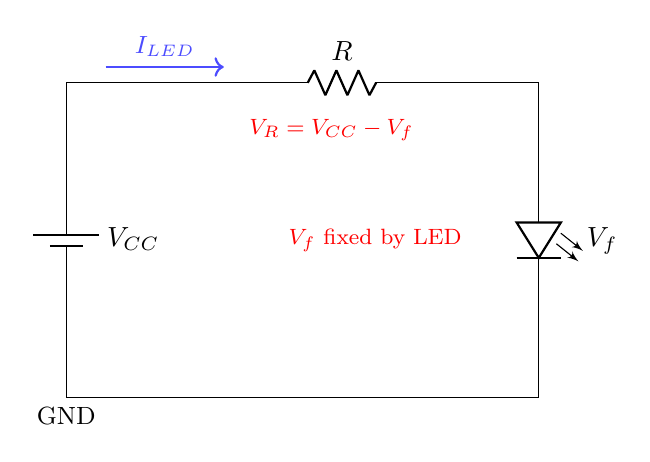
\begin{tikzpicture}[scale=1.0]
  \ctikzset{resistors/scale=0.75, diodes/scale=0.8}
  \draw (0,0) node[below]{\small GND}
    to[battery1, l_={$\Vcc$}, invert] (0,4)
    to[short] (2,4)
    %to[R, l={$R$}, v^<={$V_R$}] (5,4)
    to[R, l={$R$}] (5,4)
    to[short] (6,4)
    to[led, l={$\Vf$}] (6,0)
    to[short] (0,0);
  %% Labels
  \draw[->, thick, blue!70] (0.5,4.2) -- (2.0,4.2) node[midway,above,blue!70,font=\small]{$I_{LED}$};
  %\node[midway,above,blue!70,font=\small] at (0,4.2){$I_{LED}$};
  \node[right, font=\footnotesize, red] at (2.2,3.4) {$V_R = \Vcc - \Vf$};
  \node[right, font=\footnotesize, red] at (2.7,2.0) {$\Vf$ fixed by LED};
\end{tikzpicture}
\caption{The fundamental LED circuit. The resistor $R$ limits current by dropping
the voltage difference $V_R = \Vcc - \Vf$.}
\label{fig:basic}
\end{figure}

\subsection{The Governing Equations}

The three equations you need are all forms of Ohm's law.

\begin{conceptbox}{The Three LED Circuit Equations}
\begin{align}
  V_R &= \Vcc - \Vf \label{eq:vr} \\[6pt]
  \Iled &= \frac{V_R}{R} = \frac{\Vcc - \Vf}{R} \label{eq:iled} \\[6pt]
  R &= \frac{\Vcc - \Vf}{\Iled} \label{eq:r}
\end{align}

\noindent where:
\begin{itemize}[leftmargin=2em,itemsep=2pt]
  \item $\Vcc$ = supply voltage (V)
  \item $\Vf$ = LED forward voltage (V) --- from the datasheet
  \item $V_R$ = voltage across the resistor (V)
  \item $\Iled$ = LED current (A or mA) --- you choose this
  \item $R$ = resistor value (\si{\ohm})
\end{itemize}
\end{conceptbox}

\begin{tipbox}
The LED current $\Iled$ is the \emph{same} as the current through the resistor ---
they are in series, so only one current flows in the whole loop.
\end{tipbox}

\subsection{Worked Example: Finding $R$}

\begin{examplebox}{Example 2.1 --- Designing a red LED circuit}
\textbf{Given:}
\begin{itemize}[leftmargin=2em]
  \item Supply voltage: $\Vcc = 5.0$\volt
  \item Red LED: $\Vf = 2.2$\volt{} (typical), $\Imax = 250$\mA
  \item Desired current: $\Iled = 100$\mA
\end{itemize}

\textbf{Step 1: Find the voltage across the resistor.}
\[ V_R = \Vcc - \Vf = 5.0 - 2.2 = 2.8\volt \]

\textbf{Step 2: Calculate the required resistance.}
\[ R = \frac{V_R}{\Iled} = \frac{2.8\volt}{0.100\,\text{A}} = 28\ohm \]

\textbf{Step 3: Choose the nearest standard (E24) value.}\\
The nearest E24 value below 28\ohm{} is \textbf{27\ohm}. The nearest above is \textbf{30\ohm}.

With 27\ohm: $\Iled = 2.8 / 27 = 103.7$\mA \quad (slightly over target, but under $\Imax$)\\
With 30\ohm: $\Iled = 2.8 / 30 = 93.3$\mA \quad (slightly under target)

Either is acceptable. Choose 27\ohm{} for slightly more brightness, 30\ohm{} for
slightly more headroom below $\Imax$.
\end{examplebox}

\begin{quizbox}{Quick Check 2.1}
\quizq A blue LED has $\Vf = 2.95$\volt{} and is powered from a 5\volt{} supply.
You want $\Iled = 80$\mA. What resistor do you need?
\vspace{0.3cm}

$V_R = $ \blank \quad $R_{calc} = $ \blank \quad Nearest E24 = \blank

\vspace{0.2cm}
\textit{(See Appendix A for the answer.)}
\end{quizbox}

%%=============================================================================
\section{Understanding LED Specifications}
%%=============================================================================
\markboth{Section 3 --- Understanding Specifications}{}

Before you can design a circuit, you need to read and understand the LED datasheet.
This section explains the most important specifications.

\subsection{Forward Voltage ($\Vf$): Typical, Minimum, and Maximum}

Datasheets usually give three values for $\Vf$:

\begin{center}
\renewcommand{\arraystretch}{1.3}
\begin{tabular}{L{2cm} L{4cm} L{6cm}}
\toprule
\textbf{Value} & \textbf{Meaning} & \textbf{How to use it} \\
\midrule
$\Vf^{typ}$ & Most LEDs from this batch & Use for nominal calculations \\
$\Vf^{min}$ & Best-case (lowest voltage, highest current for given R) & Use to find maximum possible current \\
$\Vf^{max}$ & Worst-case (highest voltage, lowest current for given R) & Use to verify the LED still lights at minimum brightness \\
\bottomrule
\end{tabular}
\end{center}

\begin{warnbox}
Using only $\Vf^{typ}$ can mislead you. If $\Vf^{max}$ is much higher than $\Vf^{typ}$,
some LEDs from the production run will be noticeably dimmer than expected.
\textbf{Example:} The violet LED (row~1015 in our project) has $\Vf^{typ} = 2.8$\volt{}
but $\Vf^{max} = 4.0$\volt. With a 120\ohm{} resistor on a 5\volt{} supply:
\begin{itemize}[leftmargin=2em]
  \item At $\Vf^{typ}$: $I = (5.0 - 2.8)/120 = 18.3$\mA
  \item At $\Vf^{max}$: $I = (5.0 - 4.0)/120 = 8.3$\mA
\end{itemize}
The dimmest LEDs produce less than half the current of the brightest. Always check
the full $\Vf$ range.
\end{warnbox}

\subsection{Maximum Current ($\Imax$)}

$\Imax$ is the \emph{absolute} maximum continuous forward current. Exceeding it will
destroy the LED by overheating its junction. It is \textbf{not} a target --- it is
a hard ceiling.

\begin{tipbox}
A good operating current is \textbf{50--75\% of $\Imax$}. This gives good brightness
while keeping the junction temperature low, extending LED lifetime and maintaining
spectral stability.
\end{tipbox}

\subsection{Power Dissipation ($P_{max}$)}

Every LED also has a maximum power dissipation rating:
\[ P_{LED} = \Vf \times \Iled \]

This must stay below the datasheet's $P_{max}$. For the violet LED: $P_{max} = 120$\mW.
At $\Vf = 2.8$\volt{} and $I = 18$\mA: $P = 2.8 \times 0.018 = 50.4$\mW. Well within limit.

\begin{quizbox}{Quick Check 3.1}
\quizq A green LED has $\Vf = 2.8$\volt, $\Imax = 240$\mA, and $P_{max} = 800$\mW.
You plan to run it at $I = 150$\mA.
\begin{enumerate}[label=(\alph*), leftmargin=2.5em]
  \item What is the power in the LED?
  \item Is this within the power limit?
  \item What percentage of $\Imax$ are you using?
\end{enumerate}
\textit{(See Appendix A.)}
\end{quizbox}

\subsection{Luminous Output}

LEDs may specify brightness in several units depending on their class:
\begin{itemize}[leftmargin=2em]
  \item \textbf{lm (lumens):} Total light output. Used for power/high-brightness LEDs.
  \item \textbf{mcd (millicandela):} Intensity in a specific direction. Used for
    indicator LEDs.
  \item \textbf{mW (milliwatts):} Optical radiant power. Used for UV/IR LEDs where
    human visibility is less meaningful.
\end{itemize}

Brightness is \emph{approximately proportional to current}. Running at 50\% of $\Imax$
gives roughly 50\% of the rated luminous output.

%%=============================================================================
\section{Choosing an Operating Current}
%%=============================================================================
\markboth{Section 4 --- Choosing an Operating Current}{}

One of the most important design decisions is how hard to drive your LED. This section
introduces a systematic approach using three defined levels.

\subsection{The Three Brightness Levels}

Rather than picking current arbitrarily, define three levels as fractions of $\Imax$:

\begin{center}
\renewcommand{\arraystretch}{1.3}
\begin{tabular}{C{2cm} C{2.5cm} C{8cm}}
\toprule
\textbf{Level} & \textbf{\% of $\Imax$} & \textbf{When to use} \\
\midrule
Low    & $\approx$40\% & Calibration, testing, or when camera exposure can compensate \\
Medium & $\approx$60\% & Normal operation; good brightness with comfortable thermal margin \\
High   & $\approx$80\% & Maximum brightness needed; monitor temperature; shorter LED lifetime \\
\bottomrule
\end{tabular}
\end{center}

\begin{examplebox}{Example 4.1 --- Selecting operating currents for a green LED}
\textbf{Given:} Green LED, $\Imax = 240$\mA.

\begin{align*}
I_{Low}    &= 0.40 \times 240 = 96\mA \\
I_{Medium} &= 0.60 \times 240 = 144\mA \\
I_{High}   &= 0.80 \times 240 = 192\mA
\end{align*}

\textbf{Before accepting these, check the power budget.} If four LEDs run in parallel,
total current at Medium = $4 \times 144 = 576$\mA. If the budget is 500\mA, the
Medium target must be reduced:
\[ I_{Medium,max} = \frac{500\mA}{4\text{ LEDs}} = 125\mA \quad (52\%\text{ of }\Imax) \]
This is still a good operating point, just slightly below the 60\% guideline.
\end{examplebox}

\subsection{The Power Budget Constraint}

When multiple LEDs run in parallel, the total current is:
\begin{equation}
  I_{total} = N \times \Iled
  \label{eq:itotal}
\end{equation}

This must not exceed your supply's current limit. Always check $I_{total}$ before
finalizing a resistor value.

\begin{quizbox}{Quick Check 4.1}
\quizq You have a red LED with $\Imax = 250$\mA. You want to run 4 LEDs in parallel
from a supply limited to 500\mA.
\begin{enumerate}[label=(\alph*), leftmargin=2.5em]
  \item What is $I_{Medium}$ per LED at 60\% of $\Imax$?
  \item What is the total current at Medium? Does it fit the budget?
  \item What is the maximum per-LED current that fits the 500\mA budget?
  \item What percentage of $\Imax$ is that maximum?
\end{enumerate}
\textit{(See Appendix A.)}
\end{quizbox}

%%=============================================================================
\section{Calculating the Current-Limiting Resistor}
%%=============================================================================
\markboth{Section 5 --- Calculating the Resistor}{}

\subsection{Step-by-Step Procedure}

\begin{conceptbox}{Resistor Calculation Procedure}
\begin{enumerate}[leftmargin=2em, itemsep=4pt]
  \item Choose the desired LED current $\Iled$ (using the brightness-level approach
    from Section~4, constrained by the power budget).
  \item Compute the voltage across the resistor:
    \[ V_R = \Vcc - \Vf^{typ} \]
  \item Calculate the exact resistor value:
    \[ R_{calc} = \frac{V_R}{\Iled} \]
    \emph{(Use amperes, not milliamperes, in this formula.)}
  \item Round to the nearest \textbf{E24 standard value} (see Table~\ref{tab:e24}).
  \item Calculate the \emph{actual} current with the standard resistor:
    \[ \Iled^{actual} = \frac{V_R}{R_{E24}} \]
  \item Verify: $\Iled^{actual} < \Imax$ and $N \times \Iled^{actual} <$ budget.
\end{enumerate}
\end{conceptbox}

\subsection{The E24 Resistor Series}

Standard resistors come in the E24 series, which provides 24 values per decade.
These are the most commonly available values.

\begin{table}[H]
\centering
\caption{E24 Standard Resistor Values (multiply by any power of 10)}
\label{tab:e24}
\small
\begin{tabular}{*{12}{C{0.75cm}}}
\toprule
1.0 & 1.1 & 1.2 & 1.3 & 1.5 & 1.6 & 1.8 & 2.0 & 2.2 & 2.4 & 2.7 & 3.0 \\
3.3 & 3.6 & 3.9 & 4.3 & 4.7 & 5.1 & 5.6 & 6.2 & 6.8 & 7.5 & 8.2 & 9.1 \\
\bottomrule
\end{tabular}
\end{table}

\begin{tipbox}
To find the nearest E24 value to any calculated resistance: divide by the appropriate
power of 10 to get a value between 1 and 10, find the nearest entry in
Table~\ref{tab:e24}, then multiply back. For example, $R_{calc} = 18.7\ohm$:
divide by 10 $\to$ 1.87; nearest E24 is 1.8; multiply by 10 $\to$ \textbf{18\ohm}.
\end{tipbox}

\subsection{Full Worked Example}

\begin{examplebox}{Example 5.1 --- Complete resistor calculation for a green LED group}
\textbf{Given:}
\begin{itemize}[leftmargin=2em]
  \item Supply: $\Vcc = 5.0$\volt
  \item LED: $\Vf^{typ} = 2.80$\volt, $\Imax = 240$\mA
  \item 4 LEDs in parallel
  \item Current budget: 500\mA
  \item Target level: Medium (60\% of $\Imax$)
\end{itemize}

\textbf{Step 1: Initial target current.}
\[ \Iled^{target} = 0.60 \times 240 = 144\mA \]

\textbf{Step 2: Check power budget.}
\[ I_{total} = 4 \times 144 = 576\mA \quad > 500\mA \quad \text{(over budget!)} \]
Reduce: $\Iled^{max} = 500/4 = 125$\mA. Use $\Iled = 122$\mA (51\% of $\Imax$).

\textbf{Step 3: Voltage across resistor.}
\[ V_R = 5.0 - 2.80 = 2.20\volt \]

\textbf{Step 4: Calculate $R_{calc}$.}
\[ R_{calc} = \frac{2.20}{0.122} = 18.03\ohm \]

\textbf{Step 5: Nearest E24 value.}
$18.03\ohm \to$ divide by 10 $\to$ 1.803 $\to$ nearest E24 is 1.8 $\to$ multiply by 10
$\to$ \textbf{18\ohm}.

\textbf{Step 6: Actual current.}
\[ \Iled^{actual} = \frac{2.20}{18} = 0.1222\,\text{A} = 122.2\mA \]

\textbf{Step 7: Verify.}
\begin{itemize}[leftmargin=2em]
  \item $122.2\mA < 240\mA$ ($\Imax$) \checkmark
  \item $4 \times 122.2 = 488.9\mA < 500\mA$ (budget) \checkmark
  \item $122.2/240 = 50.9\%$ of $\Imax$ \checkmark
\end{itemize}
\end{examplebox}

%%=============================================================================
\section{Resistor Power Rating}
%%=============================================================================
\markboth{Section 6 --- Resistor Power Rating}{}

A resistor carrying current dissipates power as heat. If this exceeds the resistor's
power rating, it will overheat and drift in value (or fail). Always calculate
resistor power and select an appropriate package.

\subsection{Calculating Resistor Power}

\begin{equation}
  P_R = \Iled^2 \times R
  \label{eq:pr}
\end{equation}

\begin{examplebox}{Example 6.1 --- Resistor power for the green LED circuit}
From Example 5.1: $\Iled = 122.2$\mA, $R = 18\ohm$.
\[ P_R = (0.1222)^2 \times 18 = 0.01493 \times 18 = 0.269\Watt = 269\mW \]
\end{examplebox}

\subsection{Choosing the Right Package}

SMD resistors come in standard packages with different power ratings:

\begin{center}
\renewcommand{\arraystretch}{1.3}
\begin{tabular}{C{2cm} C{2.5cm} C{3cm} L{5cm}}
\toprule
\textbf{Package} & \textbf{Size (mm)} & \textbf{Power Rating} & \textbf{Notes} \\
\midrule
0402 & $1.0 \times 0.5$ & 0.063\Watt & Indicator LEDs ($<$63\mW in resistor) \\
0603 & $1.6 \times 0.8$ & 0.100\Watt & Low-power applications \\
0805 & $2.0 \times 1.25$ & 0.125\Watt & Moderate current \\
1206 & $3.2 \times 1.6$ & 0.25\Watt & \textbf{Recommended for power LED resistors} \\
2512 & $6.3 \times 3.2$ & 1.0\Watt & High-power applications \\
\bottomrule
\end{tabular}
\end{center}

\begin{tipbox}
Always use a package rated for \textbf{at least twice} the calculated dissipation.
This ``2$\times$ derating'' keeps the resistor cool and extends its life.
In Example~6.1, $P_R = 269$\mW: a 1206 rated 0.25\Watt{} is marginal;
consider a 2512 (1\Watt) for a comfortable margin.
\end{tipbox}

\begin{warnbox}
The most common beginner mistake in LED driver design is using a 0402 or 0603 resistor
for a power LED circuit. At 100\mA or more, the resistor can reach temperatures that
change its value, cause solder joint failures, or start a fire on a PCB. Calculate
$P_R$ for \emph{every} design.
\end{warnbox}

\begin{quizbox}{Quick Check 6.1}
\quizq Calculate the power dissipated in the resistor for each case:
\begin{enumerate}[label=(\alph*), leftmargin=2.5em]
  \item Blue LED: $R = 18\ohm$, $\Iled = 114$\mA. What is $P_R$? What package do you need?
  \item Violet LED: $R = 120\ohm$, $\Iled = 18$\mA. What is $P_R$? What package do you need?
  \item Red LED: $R = 24\ohm$, $\Iled = 117$\mA. What is $P_R$? What package do you need?
\end{enumerate}
\textit{(See Appendix A.)}
\end{quizbox}

%%=============================================================================
\section{Parallel LED Groups}
%%=============================================================================
\markboth{Section 7 --- Parallel LED Groups}{}

\subsection{Why Parallel, Not Series?}

When illuminating a surface evenly it is tempting to wire all LEDs in a single series
string with one shared resistor. This section explains in detail why that approach
fails when simple resistors are used, and what the correct alternative is.

\subsubsection{How a Series String Works in Principle}

In a series string every LED carries exactly the same current --- there is only one
path for current to flow. The resistor is calculated for the total string voltage:
\[ R = \frac{\Vcc - N \cdot \Vf}{\Iled} \]

For example, 3 red LEDs ($\Vf = 2.2$\volt) on a 12\volt{} supply at 100\mA:
\[ R = \frac{12 - (3 \times 2.2)}{0.100} = \frac{12 - 6.6}{0.100} = 54\ohm \]

This looks straightforward. In fact, series strings \emph{are} the standard approach
in commercial LED lighting --- but only when paired with a \textbf{constant-current
driver IC} that actively regulates the current regardless of what the LEDs do.
The problems described below are specific to using a simple resistor instead of a
driver IC.

\subsubsection{Problem 1: A Resistor Cannot Stabilize a Series String on 5\volt}

The fundamental role of the resistor is to absorb the difference between the supply
and the LED voltage, providing a stable current. This only works when the voltage
\emph{across the resistor} is large enough relative to the LED voltage variations.

With 3 red LEDs in series on a 5\volt{} supply:
\[ V_R = 5.0 - (3 \times 2.2) = 5.0 - 6.6 = -1.6\volt \]

The math is negative --- \textbf{the supply voltage is not high enough for 3 red LEDs
in series at all}. Only 2 red LEDs fit: $V_R = 5.0 - 4.4 = 0.6$\volt, which is barely
enough headroom for a resistor to function (recall the 1\volt{} headroom rule from
Section~8). For blue or green LEDs ($\Vf \approx 2.8$--3.0\volt), even 2 in series
exceeds 5\volt. A 5\volt{} supply can only drive series strings of \emph{one or two}
LEDs of any color --- making it impractical for groups of 4 or 6.

\subsubsection{Problem 2: Vf Production Spread Destabilizes the Whole String}

Every LED from a production batch has a slightly different $\Vf$, typically varying
$\pm$0.1--0.3\volt{} around the nominal value. In a series string, these variations
\emph{add up} across all LEDs. With 4 LEDs each having a $\pm$0.2\volt{} spread,
the total string voltage could range from $4 \times (2.0) = 8.0$\volt{} to
$4 \times (2.4) = 9.6$\volt{} --- a 1.6\volt{} range. The resistor, which must
absorb $\Vcc$ minus the string voltage, sees its share swing widely, causing a
proportional swing in current.

Because the LED I-V curve is very steep near $\Vf$, even a small change in the
\emph{net} voltage affects the current dramatically. The resistor provides damping
only in proportion to how large $V_R$ is compared to the total string voltage.
On a 5\volt{} supply with most of the voltage consumed by LEDs, $V_R$ is so small
that the resistor provides almost no stabilization at all.

\begin{examplebox}{Example 7.0a --- Vf spread in a series string vs.\ parallel}
Two red LEDs, $\Vf^{nom} = 2.2$\volt. LED~A has $\Vf = 2.1$\volt; LED~B has
$\Vf = 2.3$\volt. Supply: 5\volt.

\textbf{Series, $R = 30\ohm$ (designed for nominal):}
\[ I = \frac{5.0 - (2.1 + 2.3)}{30} = \frac{5.0 - 4.4}{30} = \frac{0.6}{30} = 20\mA \]
Now suppose both LEDs happen to be at $\Vf^{max} = 2.3$\volt:
\[ I = \frac{5.0 - 4.6}{30} = \frac{0.4}{30} = 13\mA \quad \text{(35\% less current)} \]
A 0.2\volt{} Vf shift per LED cut the current by a third because $V_R$ is tiny.

\textbf{Parallel, $R = 14\ohm$ each (designed for nominal 100\mA):}
LED~A: $I_A = (5.0 - 2.1)/14 = 2.9/14 = 207$\mA --- \emph{wait, that exceeds $\Imax$!}

\textit{Lesson:} Parallel also has issues if $V_R$ is too small.
Using a 5\volt{} supply with a proper $V_R \geq 1$\volt:
$R = (5.0 - 2.2)/0.100 = 28\ohm$.
LED~A ($\Vf = 2.1$\volt): $I_A = 2.9/28 = 103.6\mA$.
LED~B ($\Vf = 2.3$\volt): $I_B = 2.7/28 = 96.4\mA$.
Only a 7\% variation --- each LED self-regulates independently.
\end{examplebox}

\subsubsection{Problem 3: Different Colors Cannot Share a Series String}

Different LED colors have very different $\Vf$ values:
\begin{center}
\begin{tabular}{lc}
\toprule
Color & Typical $\Vf$ \\
\midrule
Red & 2.0--2.4\volt \\
Green & 2.6--3.2\volt \\
Blue & 2.8--3.2\volt \\
Violet & 2.8--4.0\volt \\
\bottomrule
\end{tabular}
\end{center}

To mix a red and a blue LED in a series string on 5\volt:
\[ V_{string} = 2.2 + 2.95 = 5.15\volt \quad > 5.0\volt \]
The combined forward voltage already exceeds the supply. No current would flow at all
--- or if the supply voltage is slightly above nominal the LED with the lower
breakdown margin could be damaged. Mixed-color series strings on 5\volt{} are
simply impossible by arithmetic.

\subsubsection{Problem 4: One Failure Kills the Whole Group}

When an LED fails, it most commonly fails \textbf{open circuit} (the bond wire
inside breaks). In a series string, one open LED breaks the only current path and
extinguishes all the others instantly. In a parallel group with individual resistors,
a failed LED removes only one branch --- the remaining LEDs continue operating,
and the failure is immediately visible in the image as one dark spot rather than
total illumination loss.

\subsubsection{Problem 5: You Cannot Adjust LEDs Independently}

In a parallel group, changing one LED's individual resistor adjusts \emph{that LED
only}. This is useful during calibration. In a series string, the single resistor
controls all LEDs together --- there is no way to compensate for one particularly
dim or bright LED without affecting the rest.

\subsubsection{When Series Strings Are the Right Choice}

It is worth understanding that commercial LED products \emph{do} use series strings
extensively --- but with a constant-current driver IC, not a resistor. The IC
continuously measures the actual current and adjusts its output voltage to keep it
exactly at the target, regardless of $\Vf$ spread, temperature, or number of LEDs.
This makes series strings efficient (no resistor heat loss) and tightly controlled.

For our circuit, which uses simple resistors and a fixed 5\volt{} supply, parallel
LEDs with individual resistors is the only practical approach. The resistor approach
trades some efficiency for simplicity, and works well as long as $V_R \geq 1$\volt.

\subsubsection{Summary of Series vs.\ Parallel (with Resistor)}

\begin{center}
\renewcommand{\arraystretch}{1.3}
\begin{tabular}{L{4.5cm} C{3cm} C{3cm}}
\toprule
\textbf{Property} & \textbf{Series + 1 resistor} & \textbf{Parallel + individual R} \\
\midrule
Works on 5\volt{} with multiple LEDs & Rarely & Yes \\
Sensitive to $\Vf$ production spread & Very (cumulative) & Low (independent) \\
Supports mixed colors & No & Yes \\
Failure of one LED & All go dark & Others continue \\
Independent per-LED adjustment & No & Yes \\
Suitable for resistor-based design & \textbf{No} & \textbf{Yes} \\
\bottomrule
\end{tabular}
\end{center}

\textbf{Individual resistors with parallel LEDs} is therefore the correct topology
for this design. Each LED is independently current-controlled regardless of its
individual $\Vf$, the 5\volt{} supply is fully compatible, colors can be freely mixed,
and individual LEDs can be trimmed or replaced without disturbing their neighbours.

\begin{figure}[H]
\centering
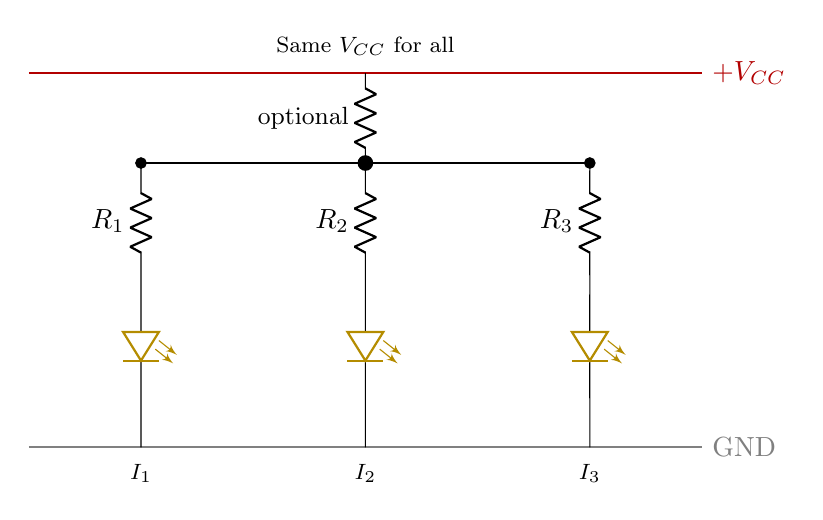
\begin{tikzpicture}[scale=0.95]
  \ctikzset{resistors/scale=0.65, diodes/scale=0.65}
  % Power rail
  \draw[red!70!black, thick] (0,5) -- (9,5) node[right]{$+\Vcc$};
  \draw[black!50, thick] (0,0) -- (9,0) node[right]{GND};

  % Rshare
  \draw (4.5,5) to[R, l={$R_{sh}$}, l_={\small optional}] (4.5,3.8)
    node[circle,fill,inner sep=2pt](bus){};

  % Bus
  \draw (1.5,3.8) -- (7.5,3.8);
  \draw[fill] (1.5,3.8) circle (2pt);
  \draw[fill] (4.5,3.8) circle (2pt);
  \draw[fill] (7.5,3.8) circle (2pt);

  % Branch 1
  \draw (1.5,3.8) to[R, l_={$R_1$}] (1.5,2.2)
    to[led, color=gold] (1.5,0.5) -- (1.5,0);

  % Branch 2
  \draw (4.5,3.8) to[R, l_={$R_2$}] (4.5,2.2)
    to[led, color=gold] (4.5,0.5) -- (4.5,0);

  % Branch 3
  \draw (7.5,3.8) to[R, l_={$R_3$}] (7.5,2.2)
    to[led, color=gold] (7.5,0.5) -- (7.5,0);

  % Labels
  \node[above, font=\footnotesize] at (4.5,5.1) {Same $\Vcc$ for all};
  \node[below, font=\footnotesize] at (1.5,-0.1) {$I_1$};
  \node[below, font=\footnotesize] at (4.5,-0.1) {$I_2$};
  \node[below, font=\footnotesize] at (7.5,-0.1) {$I_3$};
\end{tikzpicture}
\caption{Three parallel LEDs, each with its own current-setting resistor $R_1$, $R_2$,
$R_3$. An optional shared series resistor $R_{sh}$ trims the whole group simultaneously.}
\label{fig:parallel}
\end{figure}

\subsection{The Optional Shared Resistor}

A single \textbf{shared series resistor} $R_{sh}$ can be added between the supply and
the distribution bus to trim the brightness of the entire group without changing
individual resistors. It carries the full group current:
\[ I_{sh} = N \times \Iled \]

\begin{warnbox}
$R_{sh}$ carries \emph{all} the group current. At $N=4$ and $\Iled = 125$\mA,
$I_{sh} = 500$\mA. A standard 1/4\Watt{} resistor rated for 250\mA would fail.
Always use a \textbf{power-rated wirewound resistor} ($\geq$2\Watt) for $R_{sh}$,
or replace it with a wire (0\ohm) and use software exposure time to tune brightness.
\end{warnbox}

\begin{examplebox}{Example 7.1 --- Effect of $R_{sh}$ on group brightness}
Suppose 4 red LEDs ($\Vf = 2.2$\volt) each have $R_1$--$R_4 = 22\ohm$ on a 5.0\volt{} supply.

Without $R_{sh}$ ($R_{sh} = 0$):
\[ I_{LED} = \frac{5.0-2.2}{22} = \frac{2.8}{22} = 127\mA \]

Add $R_{sh} = 10\ohm$. The total resistance in series with each LED becomes:
\[ R_{total} = R_i + N \times R_{sh} / N \]
Wait --- $R_{sh}$ is in series with the whole group, not each LED individually.
The current per LED is found by:
\[ I_{LED} = \frac{\Vcc - \Vf}{R_i + R_{sh}} = \frac{5.0-2.2}{22+10} = \frac{2.8}{32} = 87.5\mA \]

Adding just 10\ohm{} of shared resistance reduced current from 127\mA to 87.5\mA
(a 31\% reduction in brightness) --- a powerful and easy group trim.
\end{examplebox}

\begin{quizbox}{Quick Check 7.1}
\quizq Four blue LEDs ($\Vf = 2.95$\volt, $R_i = 18\ohm$ each) are on a 5.0\volt{} supply.
\begin{enumerate}[label=(\alph*), leftmargin=2.5em]
  \item What is $\Iled$ with no shared resistor?
  \item What is $I_{total}$?
  \item You add $R_{sh} = 5\ohm$. What is the new $\Iled$?
  \item What power does $R_{sh}$ dissipate at the current from part (b)?
\end{enumerate}
\textit{(See Appendix A.)}
\end{quizbox}

%%=============================================================================
\section{Supply Voltage Considerations}
%%=============================================================================
\markboth{Section 8 --- Supply Voltage}{}

\subsection{Headroom: Why Supply Voltage Matters}

For stable current control, the voltage across the resistor ($V_R = \Vcc - \Vf$)
should be \textbf{at least 1\volt}. If $V_R$ is too small, tiny variations in $\Vf$
between LEDs or with temperature cause large swings in current.

\begin{examplebox}{Example 8.1 --- Why 3.3\volt{} is problematic for blue/violet LEDs}
A blue LED with $\Vf = 2.95$\volt{} on a 3.3\volt{} supply:
\[ V_R = 3.3 - 2.95 = 0.35\volt \]
With $R = 10\ohm$: $\Iled = 0.35/10 = 35$\mA.

But if this particular LED has $\Vf = 3.05$\volt{} (within production spread):
\[ \Iled = (3.3 - 3.05)/10 = 0.025\,\text{A} = 25\mA \]
That's a 29\% current variation from a 0.1\volt{} $\Vf$ change. The LED group will
have noticeable brightness differences.

On a 5\volt{} supply with $R = 22\ohm$:
\[ \Iled = (5.0 - 2.95)/22 = 93\mA \quad \text{(at } \Vf^{typ}\text{)} \]
\[ \Iled = (5.0 - 3.05)/22 = 89\mA \quad \text{(at } \Vf^{typ}+0.1\text{)} \]
Only a 4.3\% variation. The 5\volt{} supply gives much better current stability.
\end{examplebox}

\subsection{LDOs and the 5\volt{} Supply Problem}

A Linear Dropout Regulator (LDO) produces a regulated output voltage from an input.
But it requires the input to be \emph{higher} than the output by at least the
\textbf{dropout voltage} ($V_{DO}$):
\[ V_{in} \geq V_{out} + V_{DO} \]

\begin{warnbox}
\textbf{You cannot regulate 5\volt{} from a 5\volt{} supply.}
Even the best LDOs have $V_{DO} \geq 0.1$\volt. A 5.0\volt-to-5.0\volt{} LDO
would require 5.1\volt{} input minimum, and most need 5.5--6.2\volt.
If your supply is exactly 5\volt, connect the LED circuit \emph{directly} to the supply
(with bypass capacitors) rather than through an LDO.
\end{warnbox}

\begin{center}
\renewcommand{\arraystretch}{1.3}
\begin{tabular}{L{3cm} C{2cm} C{2.5cm} L{5cm}}
\toprule
\textbf{Regulator} & $V_{DO}$ & \textbf{Min Input for 5\volt{} out} & \textbf{Verdict for 5\volt{} supply} \\
\midrule
LM7805 & $\sim$2.0\volt & 7.0\volt & Cannot use on 5\volt{} supply \\
LD1117 & $\sim$1.2\volt & 6.2\volt & Cannot use on 5\volt{} supply \\
LM2940 & $\sim$0.5\volt & 5.5\volt & Cannot use on 5\volt{} supply \\
MCP1700 & $\sim$0.18\volt & 5.18\volt & Still cannot use on 5\volt{} supply \\
\textit{Direct connection} & 0 & 5.0\volt & \textbf{Correct choice} \\
\bottomrule
\end{tabular}
\end{center}

\begin{quizbox}{Quick Check 8.1}
\quizq You have a 9\volt{} DC adapter powering an LED circuit. You want to produce
a clean 5\volt{} rail for the LEDs.
\begin{enumerate}[label=(\alph*), leftmargin=2.5em]
  \item Can you use an LM7805 (needs $V_{in} \geq 7$\volt)?
  \item How much power does the LM7805 dissipate at 400\mA load current?
  \item Would you need a heatsink on the LM7805?
\end{enumerate}
\textit{(See Appendix A.)}
\end{quizbox}

%%=============================================================================
\section{The MOSFET Switch}
%%=============================================================================
\markboth{Section 9 --- The MOSFET Switch}{}

LEDs in this design are switched on and off by a microcontroller (the Raspberry Pi).
Because the GPIO pin can only supply about 16\mA, we use a transistor to switch the
much larger LED current.

\subsection{Why a MOSFET?}

A \textbf{Metal-Oxide-Semiconductor Field-Effect Transistor (MOSFET)} is ideal for
this application:
\begin{itemize}[leftmargin=2em]
  \item The gate (control input) draws virtually zero current --- it only needs a voltage.
  \item A logic-level N-channel MOSFET turns fully on with a gate voltage of 2--3\volt,
    well within the 3.3\volt{} GPIO output.
  \item When fully on, the drain-to-source resistance $R_{DS(on)}$ is very low
    (milliohms to tens of milliohms), so it drops very little voltage.
\end{itemize}

\subsection{The Gate Circuit}

Two small resistors protect the MOSFET gate:

\begin{figure}[H]
\centering
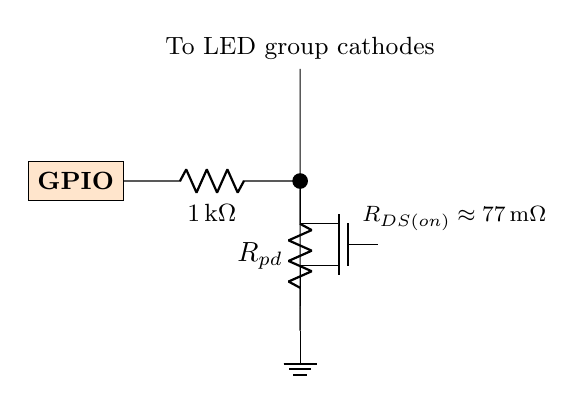
\begin{tikzpicture}[scale=0.95]
  \ctikzset{resistors/scale=0.7, transistors/scale=1.0}
  % GPIO
  \draw (0,2) node[draw, rectangle, fill=orange!20, minimum width=1cm,
    minimum height=0.5cm, font=\small\bfseries](GPIO){GPIO};
  % Gate resistor
  \draw (GPIO.east) to[R, l={$R_g$}, l_={\small 1\,k\si{\ohm}}] (3,2)
    node[circle, fill, inner sep=2pt](GN){};
  % MOSFET
  \draw (3,2) to[Tnmos, n=Q] (3,0.3);
  \draw (3,0.3) to[short] (3,0) node[ground]{};
  % Pull-down
  \draw (GN) to[R, l={\small 100\,k\si{\ohm}}, l_={$R_{pd}$}] (3,0) node[ground]{};
  % Drain (LED group connects here)
  \draw (3,3.5) node[above]{\small To LED group cathodes}
    to[short] (Q.drain);
  % Labels
  \node[font=\footnotesize, right] at (3.7,1.5) {$R_{DS(on)} \approx 77$\,m\si{\ohm}};
  \node[font=\footnotesize, left] at (-0.1,2) {};
\end{tikzpicture}
\caption{MOSFET gate circuit. $R_g$ limits the current spike when the gate capacitance
charges. $R_{pd}$ holds the gate at 0\volt{} when the GPIO pin is not actively driving it.}
\end{figure}

\begin{conceptbox}{Gate Resistor Functions}
\begin{itemize}[leftmargin=1.5em]
  \item \textbf{$R_g$ (1\,k\si{\ohm}):} The gate has a small capacitance. Without a
    series resistor, turning on the MOSFET would demand a large current spike from the
    GPIO to charge it. 1\,k\si{\ohm} limits this to $3.3\volt / 1000\ohm = 3.3$\mA,
    well within GPIO capability.
  \item \textbf{$R_{pd}$ (100\,k\si{\ohm}):} During boot, software crashes, or GPIO
    reconfiguration, the pin may float. Without $R_{pd}$, the gate could float to any
    voltage and partially turn on the LEDs at an uncontrolled time. $R_{pd}$ ensures
    the gate is firmly at 0\volt{} (LED off) unless the GPIO actively drives it high.
\end{itemize}
\end{conceptbox}

\begin{quizbox}{Quick Check 9.1}
\quizq A MOSFET with $R_{DS(on)} = 0.077\ohm$ switches a group of 4 LEDs drawing
a total of 490\mA.
\begin{enumerate}[label=(\alph*), leftmargin=2.5em]
  \item What voltage drops across the MOSFET when it is on?
  \item How much power does the MOSFET dissipate?
  \item Does it need a heatsink?
\end{enumerate}
\textit{(See Appendix A.)}
\end{quizbox}

%%=============================================================================
\section{Reading the Violet LED Datasheet: A Case Study}
%%=============================================================================
\markboth{Section 10 --- Case Study: Violet LED}{}

The violet LED used in this project (supplier row~1015, 410\,nm dominant wavelength)
illustrates several important real-world complications.

\subsection{What the Datasheet Says}

\begin{center}
\renewcommand{\arraystretch}{1.3}
\begin{tabular}{ll}
\toprule
\textbf{Parameter} & \textbf{Value} \\
\midrule
Dominant wavelength & 410\,nm \\
Forward voltage $\Vf^{typ}$ & 2.8\volt \\
Forward voltage $\Vf^{max}$ & 4.0\volt \\
Maximum current $\Imax$ & 30\mA \\
Maximum power $P_{max}$ & 120\mW \\
Package & 0603 SMD \\
\bottomrule
\end{tabular}
\end{center}

\subsection{Design Implications}

\textbf{The $\Vf$ spread is very wide:} from 2.8\volt{} to 4.0\volt{} --- a 1.2\volt{} range.
This means different LEDs from the same reel can behave very differently on the same resistor.

\textbf{The $\Imax$ is very low:} only 30\mA. This is consistent with
$P_{max} = \Vf^{max} \times \Imax = 4.0 \times 0.030 = 120$\mW. It confirms that
the datasheet is internally consistent.

\begin{examplebox}{Example 10.1 --- Full analysis for the violet LED at Medium brightness}
\textbf{Given:} $\Vcc = 5.0$\volt, $R = 120\ohm$ (chosen to give Medium brightness at typical $\Vf$).

\textbf{At $\Vf^{typ} = 2.8$\volt:}
\[ \Iled = \frac{5.0 - 2.8}{120} = \frac{2.2}{120} = 18.3\mA \]
\[ P_{LED} = 2.8 \times 18.3 = 51.2\mW \quad (<120\mW \checkmark) \]
\[ \%\Imax = 18.3/30 = 61\% \quad\text{(Medium level} \checkmark) \]

\textbf{At $\Vf^{max} = 4.0$\volt:}
\[ \Iled = \frac{5.0 - 4.0}{120} = \frac{1.0}{120} = 8.3\mA \]
\[ P_{LED} = 4.0 \times 8.3 = 33.3\mW \quad (<120\mW \checkmark) \]

\textbf{Conclusion:} The same 120\ohm{} resistor gives 8.3\mA to 18.3\mA depending
on the individual LED's $\Vf$. This is a 2.2$\times$ variation in brightness.
For a measurement application, this is acceptable because the camera exposure time
compensates for group-level brightness; within the group, brighter LEDs simply have
a lower $\Vf$.

\textbf{Why 6 LEDs instead of 4?} At only 18\mA each, a single 0603 violet LED is
much dimmer than one power LED. Using 6 multiplies total brightness by 1.5$\times$
at minimal cost, while keeping each LED safely within its 30\mA limit.
Total group current = $6 \times 18.3 = 110$\mA. Well within budget.
\end{examplebox}

%%=============================================================================
\section{Putting It All Together: Design Checklist}
%%=============================================================================
\markboth{Section 11 --- Design Checklist}{}

\begin{conceptbox}{Complete LED Driver Design Checklist}
\begin{itemize}[leftmargin=2em, itemsep=5pt, label=$\square$]
  \item \textbf{Choose LEDs} matching wavelength, package, and price goals.
  \item \textbf{Record} $\Vf^{typ}$, $\Vf^{min}$, $\Vf^{max}$, $\Imax$, $P_{max}$
    from the datasheet.
  \item \textbf{Check supply voltage headroom:} $V_R = \Vcc - \Vf^{typ} \geq 1$\volt.
  \item \textbf{Decide number of LEDs} $N$ per group.
  \item \textbf{Select operating current} $\Iled$ (target 50--75\% of $\Imax$).
  \item \textbf{Check power budget:} $N \times \Iled \leq I_{budget}$.
    Reduce $\Iled$ if necessary.
  \item \textbf{Calculate $R_{calc}$} = $(V_{CC} - \Vf^{typ}) / \Iled$.
  \item \textbf{Round to nearest E24 value} $R_{E24}$.
  \item \textbf{Calculate actual current} $\Iled^{act}$ = $(V_{CC} - \Vf^{typ}) / R_{E24}$.
  \item \textbf{Verify} $\Iled^{act} < \Imax$ and $N \times \Iled^{act} < I_{budget}$.
  \item \textbf{Calculate resistor power} $P_R = (\Iled^{act})^2 \times R_{E24}$.
  \item \textbf{Select resistor package} rated for at least $2 \times P_R$.
  \item \textbf{Check $\Vf^{max}$ scenario:} verify LED still lights at minimum current.
  \item \textbf{Select MOSFET} with $I_D > N \times \Iled^{act}$,
    logic-level gate threshold $< 3.3$\volt.
  \item \textbf{Add gate resistor} (1\,k\si{\ohm}) and pull-down (100\,k\si{\ohm}).
  \item \textbf{Add bypass capacitors} (100\,\si{\micro F} bulk + 100\,nF ceramic
    at supply input; 10\,\si{\micro F} near each LED group).
  \item \textbf{Add polyfuse} (hold current $\geq$ max group current,
    trip $\leq 1$\,A).
\end{itemize}
\end{conceptbox}

%%=============================================================================
\section{Comprehensive Exercises}
%%=============================================================================
\markboth{Section 12 --- Comprehensive Exercises}{}

Work through each exercise completely, showing all steps. Check your answers in
Appendix~A.

\begin{quizbox}{Exercise 12.1 --- Single LED, from scratch}
\exercise Design a circuit for a single blue LED on a 3.3\volt{} supply.\\
LED specs: $\Vf^{typ} = 2.75$\volt, $\Vf^{max} = 3.1$\volt, $\Imax = 30$\mA.\\
Target: Medium brightness.

\begin{enumerate}[label=(\alph*), leftmargin=2.5em]
  \item What is $\Iled^{target}$ at Medium level?
  \item What is $V_R$ using $\Vf^{typ}$?
  \item Is the headroom ($V_R$) adequate? (Is it $\geq$1\volt?)
  \item Calculate $R_{calc}$.
  \item What is the nearest E24 value?
  \item What is $\Iled^{actual}$?
  \item What is the resistor power $P_R$? What package do you need?
  \item What is $\Iled$ at $\Vf^{max}$? Does the LED still light?
\end{enumerate}
\end{quizbox}

\begin{quizbox}{Exercise 12.2 --- Power budget constraint}
\exercise You have four red LEDs ($\Vf = 2.2$\volt, $\Imax = 250$\mA) on a 5\volt{}
supply. Your current budget is 400\mA (not 500\mA --- this supply is more constrained).

\begin{enumerate}[label=(\alph*), leftmargin=2.5em]
  \item What is the maximum allowed current per LED?
  \item What percentage of $\Imax$ is that?
  \item Calculate $R_{calc}$ for this current.
  \item Round to E24. What is $\Iled^{actual}$ and $I_{total}$?
  \item Calculate $P_R$. What package?
  \item Now recalculate for Low and High brightness. Can you reach High within budget?
\end{enumerate}
\end{quizbox}

\begin{quizbox}{Exercise 12.3 --- Forward voltage spread analysis}
\exercise A green LED has $\Vf^{typ} = 2.80$\volt{} and $\Vf^{max} = 3.20$\volt.
You choose $R = 18\ohm$ on a 5.0\volt{} supply.

\begin{enumerate}[label=(\alph*), leftmargin=2.5em]
  \item What is $\Iled$ at $\Vf^{typ}$?
  \item What is $\Iled$ at $\Vf^{max}$?
  \item What is the ratio $I(\Vf^{max}) / I(\Vf^{typ})$ expressed as a percentage?
  \item Is the headroom ($V_R$ at $\Vf^{max}$) at least 1\volt?
  \item Repeat for a supply of 3.3\volt{} with $R = 2\ohm$. What do you notice?
\end{enumerate}
\end{quizbox}

\begin{quizbox}{Exercise 12.4 --- Full four-channel design}
\exercise Design resistors for all four channels of a color analyzer. Supply: 5.0\volt,
budget: 500\mA per group. Use Medium brightness (but cap at budget limit). LEDs:

\begin{center}
\begin{tabular}{lllll}
\toprule
Channel & $\Vf^{typ}$ & $\Imax$ & $N$ LEDs & Notes \\
\midrule
Violet & 2.80\volt & 30\mA & 6 & Estimated $\Imax$ \\
Blue   & 2.95\volt & 240\mA & 4 & \\
Green  & 2.80\volt & 240\mA & 4 & \\
Red    & 2.20\volt & 250\mA & 4 & \\
\bottomrule
\end{tabular}
\end{center}

For each channel: (a) target current per LED, (b) $R_{calc}$, (c) $R_{E24}$,
(d) $\Iled^{actual}$, (e) $I_{total}$, (f) $P_R$ and minimum package.
\end{quizbox}

\begin{quizbox}{Exercise 12.5 --- Resistor sizing judgment}
\exercise For each scenario, state whether the proposed resistor package is adequate,
marginal, or dangerously undersized, and explain why.

\begin{enumerate}[label=(\alph*), leftmargin=2.5em]
  \item $\Iled = 20$\mA, $R = 100\ohm$, package = 0402 (63\mW rating)
  \item $\Iled = 120$\mA, $R = 18\ohm$, package = 0603 (100\mW rating)
  \item $\Iled = 115$\mA, $R = 24\ohm$, package = 1206 (250\mW rating)
  \item $\Iled = 80$\mA, $R = 20\ohm$, package = 0805 (125\mW rating)
\end{enumerate}
\end{quizbox}

%%=============================================================================
%% APPENDIX
%%=============================================================================
\appendix
\setcounter{section}{0}
\renewcommand{\thesection}{A}

\section{Answer Key}
\markboth{Appendix A --- Answer Key}{}

\subsection*{Quick Check 2.1}
\begin{answerbox}{Answer --- Quick Check 2.1}
Blue LED, $\Vf = 2.95$\volt, $\Vcc = 5$\volt, target $\Iled = 80$\mA.

\[ V_R = 5.0 - 2.95 = 2.05\volt \]
\[ R_{calc} = \frac{2.05}{0.080} = 25.6\ohm \]

Nearest E24: $25.6\ohm \to$ divide by 10 $\to$ 2.56 $\to$ nearest E24 values are 2.4 and
2.7. Distance: $|2.56-2.4|=0.16$; $|2.56-2.7|=0.14$. Nearest is \textbf{2.7}
$\to$ \textbf{27\ohm}.

Actual current: $\Iled = 2.05/27 = 75.9$\mA (slightly under target, fine).
\end{answerbox}

\subsection*{Quick Check 3.1}
\begin{answerbox}{Answer --- Quick Check 3.1}
$\Vf = 2.8$\volt, $\Imax = 240$\mA, $P_{max} = 800$\mW, $I = 150$\mA.

(a)~$P_{LED} = 2.8 \times 0.150 = 0.42$\Watt $= 420$\mW.

(b)~$420\mW < 800\mW$ --- within limit. \checkmark

(c)~$150/240 = 62.5\%$ of $\Imax$.
\end{answerbox}

\subsection*{Quick Check 4.1}
\begin{answerbox}{Answer --- Quick Check 4.1}
Red LED, $\Imax = 250$\mA, 4 LEDs, 500\mA budget.

(a)~$I_{Medium} = 0.60 \times 250 = 150$\mA per LED.

(b)~$I_{total} = 4 \times 150 = 600$\mA. \textbf{Exceeds 500\mA budget.}

(c)~$I_{max,LED} = 500/4 = 125$\mA per LED.

(d)~$125/250 = 50\%$ of $\Imax$. Still a reasonable operating point.
\end{answerbox}

\subsection*{Quick Check 6.1}
\begin{answerbox}{Answer --- Quick Check 6.1}
(a)~Blue: $P_R = (0.114)^2 \times 18 = 0.01300 \times 18 = 234$\mW.
Need 1206 (250\mW) minimum; 2$\times$ derating suggests 2512 (1\Watt).

(b)~Violet: $P_R = (0.018)^2 \times 120 = 0.000324 \times 120 = 38.9$\mW.
0402 (63\mW) is adequate; 0603 comfortable.

(c)~Red: $P_R = (0.117)^2 \times 24 = 0.01369 \times 24 = 328$\mW.
Exceeds 1206 (250\mW) rating --- use \textbf{2512 (1\Watt)} or use
$R = 27\ohm$ to reduce current slightly.
\end{answerbox}

\subsection*{Quick Check 7.1}
\begin{answerbox}{Answer --- Quick Check 7.1}
Blue LEDs, $\Vf = 2.95$\volt, $R_i = 18\ohm$, $\Vcc = 5.0$\volt, $N=4$.

(a)~$\Iled = (5.0 - 2.95)/18 = 2.05/18 = 113.9$\mA.

(b)~$I_{total} = 4 \times 113.9 = 455.6$\mA.

(c)~With $R_{sh} = 5\ohm$: $\Iled = (5.0-2.95)/(18+5) = 2.05/23 = 89.1$\mA.

(d)~$P_{Rsh} = (0.4556)^2 \times 5 = 0.2076 \times 5 = 1.04$\Watt.
Must use a wirewound resistor rated $\geq$2\Watt.
\end{answerbox}

\subsection*{Quick Check 8.1}
\begin{answerbox}{Answer --- Quick Check 8.1}
9\volt{} supply, LM7805 (needs $V_{in} \geq 7$\volt), 400\mA load.

(a)~Yes. 9\volt{} $\geq$ 7\volt. The LM7805 \textbf{can} be used.

(b)~Power dissipated in LM7805 $= (V_{in} - V_{out}) \times I = (9-5) \times 0.4 = 4 \times 0.4 = 1.6$\Watt.

(c)~\textbf{Yes, a heatsink is required.} The LM7805 in TO-220 can only dissipate
about 1\Watt{} without a heatsink in free air. At 1.6\Watt{} it will overheat
and go into thermal shutdown. Use a clip-on TO-220 heatsink.
\end{answerbox}

\subsection*{Quick Check 9.1}
\begin{answerbox}{Answer --- Quick Check 9.1}
IRL540N MOSFET, $R_{DS(on)} = 0.077\ohm$, $I = 490$\mA.

(a)~$V_{DS} = I \times R_{DS(on)} = 0.490 \times 0.077 = 37.7\,\si{mV}$. Negligible.

(b)~$P_{FET} = I^2 \times R_{DS(on)} = (0.490)^2 \times 0.077 = 0.240 \times 0.077 = 18.5$\mW.

(c)~No heatsink needed. 18.5\mW is far below the TO-220 package's thermal limit.
The device will barely warm up.
\end{answerbox}

\subsection*{Exercise 12.1}
\begin{answerbox}{Answer --- Exercise 12.1}
Blue LED, $\Vf^{typ}=2.75$\volt, $\Vf^{max}=3.1$\volt, $\Imax=30$\mA, $\Vcc=3.3$\volt.

(a)~$I_{Medium} = 0.60 \times 30 = 18$\mA.

(b)~$V_R = 3.3 - 2.75 = 0.55$\volt.

(c)~\textbf{Headroom is inadequate.} $0.55\volt < 1\volt$. Current will be very sensitive
to $\Vf$ variation. This supply-LED combination is marginal at best.

(d)~$R_{calc} = 0.55 / 0.018 = 30.6\ohm$.

(e)~Nearest E24: \textbf{30\ohm}.

(f)~$\Iled = 0.55/30 = 18.3$\mA.

(g)~$P_R = (0.0183)^2 \times 30 = 0.000335 \times 30 = 10.0$\mW. 0402 is fine (63\mW rated).

(h)~At $\Vf^{max} = 3.1$\volt: $V_R = 3.3-3.1 = 0.2$\volt.
$\Iled = 0.2/30 = 6.7$\mA. The LED is very dim but still lit.
\textit{Key lesson:} a 3.3\volt{} supply is too close to the $\Vf$ of blue LEDs for
stable, repeatable results. Use 5\volt{} if possible.
\end{answerbox}

\subsection*{Exercise 12.2}
\begin{answerbox}{Answer --- Exercise 12.2}
Red LED, $\Vf=2.2$\volt, $\Imax=250$\mA, $N=4$, $\Vcc=5$\volt, budget=400\mA.

(a)~$I_{max/LED} = 400/4 = 100$\mA.

(b)~$100/250 = 40\%$ of $\Imax$. This is the Low level.

(c)~$R_{calc} = (5.0-2.2)/0.100 = 2.8/0.100 = 28\ohm$.

(d)~Nearest E24: \textbf{27\ohm}. $\Iled = 2.8/27 = 103.7$\mA.
$I_{total} = 4 \times 103.7 = 414.8$\mA. Slightly over 400\mA; use \textbf{30\ohm}
instead. $\Iled = 2.8/30 = 93.3$\mA. $I_{total} = 373.3$\mA. \checkmark

(e)~$P_R = (0.0933)^2 \times 30 = 261$\mW. Use 1206 (250\mW) or larger.

(f)~Low with 30\ohm: done above.\\
Medium (60\%): $I_{target}=150$\mA; $I_{total}=600$\mA --- \textbf{exceeds 400\mA budget}.
Medium must be capped at $100$\mA (same as Low for this budget).\\
High (80\%): $I_{target}=200$\mA; $I_{total}=800$\mA --- far over budget.
\textbf{High is not achievable within a 400\mA budget with 4 LEDs at $\Imax=250$\mA.}
The budget limits this design to approximately the Low operating level.
\end{answerbox}

\subsection*{Exercise 12.3}
\begin{answerbox}{Answer --- Exercise 12.3}
Green LED, $\Vf^{typ}=2.80$\volt, $\Vf^{max}=3.20$\volt, $R=18\ohm$, $\Vcc=5.0$\volt.

(a)~$\Iled(\Vf^{typ}) = (5.0-2.80)/18 = 2.20/18 = 122.2$\mA.

(b)~$\Iled(\Vf^{max}) = (5.0-3.20)/18 = 1.80/18 = 100.0$\mA.

(c)~$100.0/122.2 = 81.8\%$. The dimmest LED produces 82\% of the brightest LED's
output --- an 18\% variation. Acceptable for most applications.

(d)~$V_R$ at $\Vf^{max} = 5.0-3.2 = 1.8$\volt \,$> 1$\volt. \checkmark Adequate headroom.

(e)~At 3.3\volt{} with $R=2\ohm$:
$\Iled(\Vf^{typ}) = (3.3-2.8)/2 = 0.5/2 = 250$\mA. Exceeds $\Imax$!
$\Iled(\Vf^{max}) = (3.3-3.2)/2 = 0.1/2 = 50$\mA.
The ratio is $50/250 = 20\%$: a 5$\times$ variation. \textbf{The low-voltage supply
makes the circuit extremely sensitive to $\Vf$ variation.}
\end{answerbox}

\subsection*{Exercise 12.4}
\begin{answerbox}{Answer --- Exercise 12.4}
\small
\begin{center}
\renewcommand{\arraystretch}{1.4}
\begin{tabular}{L{1.3cm} C{1.4cm} C{1.1cm} C{1.2cm} C{1.2cm} C{1.3cm} C{1.3cm} L{2.2cm}}
\toprule
\textbf{Ch.} & \textbf{$I_{target}$} & \textbf{$R_{calc}$} & \textbf{$R_{E24}$} & \textbf{$I_{act}$} & \textbf{$I_{tot}$} & \textbf{$P_R$} & \textbf{Package} \\
\midrule
Violet & 18.0\mA & 122.2\ohm & 120\ohm & 18.3\mA & 110\mA & 39.9\mW & 0402 \\
Blue   & 114\mA* & 18.0\ohm & 18\ohm & 113.9\mA & 455\mA & 234\mW & 1206 \\
Green  & 122\mA* & 18.0\ohm & 18\ohm & 122.2\mA & 489\mA & 268\mW & 1206 \\
Red    & 117\mA* & 23.9\ohm & 24\ohm & 116.7\mA & 467\mA & 327\mW & 2512 \\
\bottomrule
\end{tabular}
\end{center}
\normalsize
*Budget-constrained: $500\mA / 4 = 125\mA$ max; round to nearest E24 that keeps
$I_{total} \leq 500$\mA. Violet: $\Imax=30$\mA, Medium $= 0.60 \times 30 = 18$\mA; 6 LEDs
$\times 18.3 = 110$\mA. Red: 22\ohm gives $I_{total}=509$\mA (over); use 24\ohm.
\end{answerbox}

\subsection*{Exercise 12.5}
\begin{answerbox}{Answer --- Exercise 12.5}
(a)~$P_R = (0.020)^2 \times 100 = 40$\mW. 0402 rated 63\mW: $40 < 63$. \textbf{Adequate},
though 2$\times$ derating suggests 0603 for comfort.

(b)~$P_R = (0.120)^2 \times 18 = 259$\mW. 0603 rated 100\mW: $259 \gg 100$.
\textbf{Dangerously undersized.} The resistor will overheat and fail. Use 1206 at minimum.

(c)~$P_R = (0.115)^2 \times 24 = 317$\mW. 1206 rated 250\mW: $317 > 250$.
\textbf{Marginal to undersized.} Exceeds the 1206 rating. Use 2512 (1\Watt) for 2$\times$
derating. At minimum, increase $R$ to reduce current slightly.

(d)~$P_R = (0.080)^2 \times 20 = 128$\mW. 0805 rated 125\mW: $128 \approx 125$.
\textbf{Marginal.} Barely at the limit; 2$\times$ derating is violated.
Use 1206 for safety.
\end{answerbox}

\end{document}
